%----------------------------------------------------------------------------
\chapter{Háttérismeretek}

\section{Biometrikus azonosítás}

A biometria az emberek fizikai jellemzőinek mérésével és elemzésével foglalkozik. Alkalmazását tekintve három területet különböztetünk meg:

\begin{itemize}
	\item Felhasználó ellenőrzés: Az azonosító rendszer a biometrikus adatot egy, korábban vetthez hasonlítja. Ez alapján dönt, hogy a felhasználó hozzáférhet-e a kívánt erőforráshoz. Ilyen egy ujjlenyomat-olvasóval ellátott mobiltelefonon a képernyőzár feloldása. A felhasználó ellenőrzés arra ad választ, hogy az illető az-e akinek mondja magát.
	\item Felhasználó azonosítás: Az azonosító rendszer a biometrikus adatot több korábban vett mintához hasonlítja és arra ad választ, hogy ki a felhasználó; azaz beletartozik-e a korábban eltárolt biometrikus adatokból álló csoportba vagy nem. Ilyen lehet például egy ujjlenyomat-leolvasóval ellátott beléptetőrendszer cégek esetében.
	\item Duplikátum detektálás: Annak ellenőrzése, hogy egy felhasználó egynél többször szerepel-e egy adatbázisban. Csalások, például szociális támogatást többször igénylők kiszűrésére használják.
\end{itemize}

Az első biometrikus azonosítási eljárás az ujjlenyomatvételen alapuló személyiségazonosítás volt, amely a modern kriminalisztika világában terjedt el, de manapság már megtalálható okostelefonokban, biometrikus beléptetőrendszerekben is.

A biometrikus azonosítást az ún. biometrikus azonosító rendszer végzi el. A folyamat során a biometrikus azonosító rendszer mintát vesz az azonosítandó egyén egy vagy több előre meghatározott fizikai jellemzőjéről, és ezekről digitális lenyomatokat képez. Az első, regisztrációs fázisban a biometrikus minta lenyomatát a rendszer egy adatbázisban eltárolja, majd később az azonosítás során az aktuális mintát összeveti a korábban rögzítettel és dönt az egyezésről. Ahhoz, hogy az ember egy fizikai jellemzőjét biometrikus adatként használhassuk, a következő elvárásokat támasztjuk vele szemben:

\begin{itemize}
	\item Általánosság: A biometrikus adattal minden egyénnek rendelkeznie kell.
	\item Egyediség: A biometrikus adatnak egyedinek kell lennie a releváns populáción belül.
	\item Állandóság: A biometrikus adat nem, vagy csak keveset változzon az idő eltetével.
	\item Mérhetőség: Az biometrikus adat az egyén részéről legyen könnyen mérhető testi adottság.
	\item Teljesítmény: A biometrikus azonosító rendszerek teljesítménye: gyorsaság, pontosság, technológia.
	\item Elfogadottság: A releváns populáción belül a mérési eljárás mennyire elfogadott (emberi méltóság megőrzése).
	\item Biztonság: Mennyire nehéz utánozni, hamisítani a biometrikus adatot?
\end{itemize}

A biometrikus adat lehet fiziológiai (DNS, arc, ujjlenyomat, írisz) vagy viselkedési (hang, írás, gesztusok). Mivel ezek az adatok statisztikai jellegűek, megbízhatóságuk változó. Minél több adat van egy mintában, annál egyedibb, és minél nagyobb a releváns populáció (eltárolt minták összessége), annál valószínűbb, hogy találunk két hasonló mintát. Ennek elkerülésére manapság terjednek a multimódusú biometrikus azonosító rendszerek, amelyek több biometrikus adatot felhasználva végzik ez az ellenőrzés, azonosítás és duplikátum detektálás feladatát. 


\section{Beszélőfelismerés}

Az emberi kommunikáció során fontos feladat a beszélő partner felismerése. A telekommunikációs technológia fejlődése miatt elterjedt a telefonon vagy interneten történő hangalapú kommunikáció; a telefonos felhasználófelismerés mint biometrikus azonosítási módszer megjelent már banki alkalmazásokban, call centerekben és az elektronikus kereskedelemben is (mobiltelefonos vásárlás). Az elektronikus kommunikáció során sokszor csak a beszélő hangjára hagyatkozhatunk, az alapján ismerhetjük fel az illetőt. A beszélőfelismerést háromféle módon végezhetjük:

\begin{itemize}
	\item Naiv beszélőfelismerés: Az emberi, naiv beszélőfelismerés során az ismerős hangokat meglepően nagy pontossággal ismerjük fel.
	\item Törvényszéki beszélőfelismerés: A törvényszéki szakértői vizsgálat eredménye.
	\item Automatikus beszélőfelismerés: A beszélőfelismerést számítógépes rendszer végzi.
\end{itemize}

A beszélőfelismerés alatt három szűkebb fogalmat értünk. Ha a folyamat során az ismeretlen beszélőről azt ellenőrizzük, hogy az-e akinek állítja magát beszélő ellenőrzésről van szó. Beszélő szegmentáláskor a hangmintát homogén csoportokra bontjuk a beszélő személye alapján. Végül beszélő azonosításról beszélünk, ha az illető hangját rögzített hangok egy csoportjával vetjük össze és azt szeretnénk eldönteni, hogy melyikhez hasonlít a legjobban. Utóbbi felveti a kérdést, hogy mi történik ha a beszélő nem tagja a csoportnak. 

Emiatt megkülönböztetjük a nyitott és zárt halmazú beszélőazonosítást. Utóbbi esetén csak olyan beszélőket ismerünk fel, akikről van hangminta az adatbázisban, míg az előbbinél ismeretlen beszélők is megjelenhetnek, így ezt is kezelni kell.

A beszélőfelismerés továbbá lehet szöveg-függő és szöveg-független attól függően, hogy a felismerő rendszer egy előre meghatározott mondatot vár, vagy bármilyen hangminta alapján működik.

\section{Az automatikus beszélőfelismerés története}

Az automatikus beszélőfelismerést egy számítógépes program végzi emberi beavatkozás nélkül. Az első automatikus beszédfelismerő rendszert a Texas Instruments fejlesztetése volt és 1977-ben publikálták. A rendszer szövegfüggő beszélőellenőrzésre volt képes és az évek során a téves elutasítási és elfogadási rátája 1$\%$ alatt maradt. A hetvenes évek óta a a beszélőazonosító és ellenőrző rendszerek rengeteget fejlődtek kezdve a vektor kvantálástól kezdve a GMM modelleken át a mély neurális hálókig. 

\begin{figure}[!ht]
	\centering
	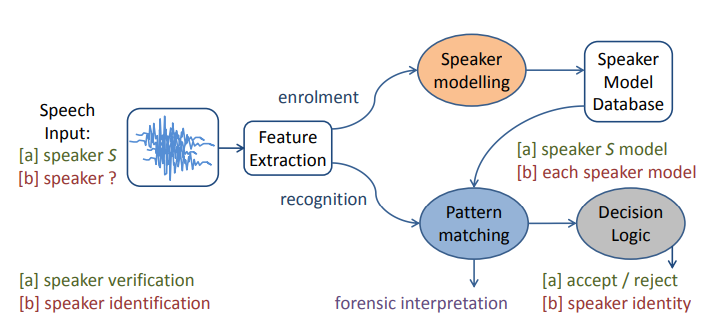
\includegraphics[width=150mm, keepaspectratio]{figures/automatic_speaker_recognition.png}
	\caption{Automatikus beszélőfelismerő rendszer architektúrája.}
	\label{fig:automatic_speaker_recognition}
\end{figure}

Az automatikus beszélőfelismerő általános működését az alábbi (!) ábra szemlélteti. A beszélő-ellenőrzés és beszélőazonosítás során is az első lépés rögzített \emph{jellemzők kinyerése}. Ezután az első, \emph{tanító fázisban} referencia modelleket készítünk az egyes beszélőkhöz a jellemzők alapján, amelyeket eltároljuk a beszélő adatbázisban. Beszélő-ellenőrzés esetén ebben a fázisban egy küszöbérték is meghatározásra kerül. \emph{Teszt fázisban} a rendszer kinyeri ugyanazokat a jellemzőket az aktuális hangmintából, majd \emph{jellemző összehasonlítás} történik.

\begin{enumerate}
	\item beszélő-ellenőrzés esetén megkeresi az ellenőrizendő személyhez tartozó modellt az adatbázisban és összehasonlítja az aktuális jellemzőkkel. Ha az eredmény a küszöbszint felett van, a rendszer egyezést mutat.
	\item beszélőazonosítás esetén az aktuális jellemzőket az összes modellel összehasonlítja, majd a legjobb egyezés mellett dönt. 
\end{enumerate}

\subsection{Jellemző kinyerés}
A jellemző kinyerés célja a dimenzió csökkentése és a beszélőspecifikus információk kinyerése. Mivel a beszéd komplex jel, a beszélő azonosítása szempontjából felesleges információkat is hordoz. Ilyen például a környezet és a csatorna zaja. A kinyert jellemzőket a hangminta terjedelme alapján osztályozzuk. \emph{Rövidtávú jellemzők} a 20-30 ms-os keretekből kinyert mel-frekvenciás és lineáris prediktív kepsztrális együtthatók (MFCC és LPCC). A \emph{prozódikus jellemzők} kinyerése 100 ms-os terjedelemben történik és a beszéd ritmusát, a hangmagasságot és a sebességet jellemzik. A hosszútávú jellemzőket a jel akár perc hosszú kereteiből nyerjük ki. Ezek képesek reprezentálni a beszélő akcentusát illetve a szavak szemantikáját és az idiolektust.

A beszélőfelismerő rendszerek teljesítményét javította, ha a jellemzőket csak
a hangminta azon részeiből nyerték ki, amikben beszéd is volt. Erre alkalmazott technika a \emph{Voice Activation Detection} (\emph{VAD}).

\subsection{Jellemző normalizálás}

Jellemzőkinyerés során próbáljuk kiszűrni a beszélő szempontjából értékes részéket, ugyanakkor nincs tökéletes jellemző, amely ne változna a környezet hatására. Ezt a változást segítik minimalizálni a normalizálási módszerek.

\subsection{Beszélő modellek}

Kezdetben a vektor kvantálás volt az elterjed modellezési módszer, amit később a \emph{Gaussian Mixture Model} (\emph{GMM}) váltott fel. A GMM egy adathalmazt több normális eloszlás keverékeként ír le és képes nem felügyelt módon klaszterezni az adatokat. Egy beszélőhöz egy valószínűségi sűrűségfüggvényt rendel, amely különböző pontokban kiértékelve (például teszt fázisban a beszélőtől kinyert jellemzők) egy valószínűséget ad a két beszélő hasonlóságára.

A GMM megközelítés főleg beszélőazonosításra alkalmas. Beszélő-ellenőrzéshez szükség volt egy másik modellre is, ami képes leírni minden más beszélőt az ellenőrizendőn kívül. Erre adott megoldást az \emph{Universal Background Model} (\emph{UBM}). Később jobb teljesítményt értek el, ha a teszt fázisban a beszélőkkel először UBM modelleket tanítottak és ezekből származtattak GMM-eket. Ezt nevezik GMM-UBM módszernek.

Mivel a tanító és teszt hangminták eltérő hosszúságúak lehetnek, szükség volt egy fix hosszúságú reprezentációra, ezt oldották meg a GMM szupervektorok, amelyeket az akkori megközelítés szerint szupport-vektor gépekkel vagy faktoranalízissel használtak.

Az utóbbi két módszer előnyeit kombinálva megszületett az $i-vektorok$, amelyet követve eljutunk a mai state-of-the-art módszerhez, a mély neurális hálózatokhoz (DNN).

\section{Korábbi eredmények}



\begin{table}[!ht]
	\resizebox{\textwidth}{!}{%
	\begin{tabular}{*7l} \toprule
		\bfseries Szerző (év)
		& \bfseries Szervezet
		& \bfseries Adatbázis
		& \bfseries Módszer
		& \bfseries Jellemzők
		& \bfseries \begin{tabular}{@{}l@{}} Hang \\ típusa \end{tabular}
		& \bfseries Pontosság \\ \midrule
		
		\begin{tabular}{@{}l@{}} Douglas A. Reynolds  \\  (1995) \end{tabular}
		& \begin{tabular}{@{}l@{}} Lincoln  \\  Laboratory \end{tabular}
		& 49
		& MFCC 
		& \begin{tabular}{@{}l@{}} rövid \\ kifejezések \end{tabular} 
		& telefon 
		& 96.8 \% \\
		
		\begin{tabular}{@{}l@{}} Rabah W.  \\  (2004) \end{tabular}
		& \begin{tabular}{@{}l@{}} King Abdulaziz  \\  University \end{tabular}
		& 20
		& \begin{tabular}{@{}l@{}} SVD-alapú   \\  algoritmus \end{tabular}
		& LPC/Cepstral
		& iroda
		& 94 \% \\
		
		\begin{tabular}{@{}l@{}} Yang Shao  \\  (2008) \end{tabular}
		& \begin{tabular}{@{}l@{}} Ohio State  \\  University \end{tabular}
		& 34 
		& GFCCs 
		& hallási jellemzők
		& telefon
		& \~{}99.33 \% \\
		
		\begin{tabular}{@{}l@{}} P. Krishnamoorthy  \\  (2011) \end{tabular}
		& TIMIT
		& 100 
		& GMM-UBM 
		& MFCC
		& labor
		& 80 \% \\
		
		\begin{tabular}{@{}l@{}} Alfredo Maesa  \\  (2012) \end{tabular}
		& Voxforge.org
		& 250 
		& MFCC 
		& \begin{tabular}{@{}l@{}} spektrális \\ jellemzők \end{tabular} 
		& \begin{tabular}{@{}l@{}} beszéd- \\ adatbázis \end{tabular} 
		& > 96 \% \\

		\begin{tabular}{@{}l@{}} Sharada V. Chougule  \\  (2015) \end{tabular}
		& \begin{tabular}{@{}l@{}} Finolex Academy  \\  of Management \\ and Technology \end{tabular}
		& 97 
		& NDSF 
		& spektrális
		& labor
		& \~{}98-100 \% \\
		
	\bottomrule
	\end{tabular}}
	\centering
	\caption{Korábbi eredmények szövegfüggetlen beszélőazonosítás terén.}
	\label{fig:timit-dialects}
\end{table}


